\documentclass[11pt, a4paper]{article}

% Fonts and Encoding
\usepackage[utf8]{inputenc}
\usepackage[T1]{fontenc}
\usepackage{lmodern}

% Math and Symbols
\usepackage{amsmath, amssymb, amsthm, amsfonts, mathrsfs, mathtools}

% Layout and Geometry
\usepackage{geometry}
\geometry{a4paper, margin=1in}

% Formatting and Graphics
\usepackage{graphicx, xcolor, enumitem, booktabs, array, tabularx}

% TikZ for Illustrations
\usepackage{tikz}
\usetikzlibrary{arrows.meta, positioning, shapes.geometric, calc, backgrounds, matrix}

% Clickable Links and TOC
\usepackage{hyperref}
\hypersetup{
    colorlinks=true,
    linkcolor=blue,
    filecolor=magenta,      
    urlcolor=cyan,
    pdftitle={Advanced Mathematics Topic},
}

% Theorem Environments
\newtheorem{theorem}{Theorem}[section]
\newtheorem{lemma}[theorem]{Lemma}
\newtheorem{proposition}[theorem]{Proposition}
\newtheorem{corollary}[theorem]{Corollary}
\theoremstyle{definition}
\newtheorem{definition}{Definition}[section]
\newtheorem{axiom}{Axiom}[section]
\newtheorem{example}{Example}[section]
\theoremstyle{remark}
\newtheorem{remark}{Remark}[section]

% Custom Commands (Enforced standard notation)
\newcommand{\R}{\mathbb{R}}
\newcommand{\N}{\mathbb{N}}
\newcommand{\Z}{\mathbb{Z}}
\newcommand{\Q}{\mathbb{Q}}
\newcommand{\E}{\mathbb{E}}
\newcommand{\Prob}{\mathbb{P}}
\newcommand{\F}{\mathcal{F}}

\title{Advanced Abstract Mathematics: Equivalence Relations, Partitions, and Rigorous Proofs}
\author{Tashfeen Omran}
\date{October 29, 2026}

\begin{document}

\maketitle
\tableofcontents
\newpage

\section{Concept Checklist \& Question Mapping}

The following table maps the theoretical concepts and proof techniques extracted from the foundational text to the 30 rigorous practice problems provided in this document.

\vspace{1em}
\renewcommand{\arraystretch}{1.5}
\noindent
\begin{tabularx}{\textwidth}{l X l}
\toprule
\textbf{ID} & \textbf{Concept / Proof Technique} & \textbf{Associated Problems} \\
\midrule
C1 & Abstract Property Verification (Reflexivity, Symmetry, Transitivity) & 1, 2, 3, 4, 5 \\
C2 & Partition Mapping \& Equivalence Classes & 6, 7, 8, 9, 10 \\
C3 & Combinatorial \& Meta-Relational Arguments & 11, 12, 13, 14, 15 \\
C4 & The ``Zero-Addition'' Trick \& Algebraic Bridges & 16, 17 \\
C5 & Parity and Divisibility Translation & 1, 4, 20 \\
C6 & Symmetry as a Path-Reverser & 11, 12, 14 \\
C7 & Well-Defined Operations on Quotient Sets & 18, 19, 20 \\
C8 & Real-World Modeling (MDP Bisimulation, Asset Clustering, ML) & 21, 22, 23, 24, 25 \\
C9 & Diagnostic Testing / Finding Flaws (Empty Domain, Div by Zero) & 26, 27, 28, 29, 30 \\
\bottomrule
\end{tabularx}
\vspace{1em}

\newpage

\section{Problem Set: 30 Rigorous Mathematical Problems}

\subsection{Abstract Property Verification}
\begin{enumerate}[label=\textbf{\arabic*.}]
    \item Let $R$ be a relation on $\Z$ defined by $xRy \iff 5 \mid (2x + 3y)$. Prove that $R$ is an equivalence relation.
    \item Let $R$ be a relation on $\R^2$ defined by $(x_1, y_1) R (x_2, y_2) \iff x_1^2 + y_1^2 = x_2^2 + y_2^2$. Prove that $R$ is an equivalence relation and geometrically describe its equivalence classes.
    \item Let $f: X \to Y$ be a function. Define a relation $R$ on $X$ by $x_1 R x_2 \iff f(x_1) = f(x_2)$. Prove that $R$ is an equivalence relation.
    \item Let $R$ be a relation on $\Z$ defined by $xRy \iff x^2 \equiv y^2 \pmod 7$. Prove that $R$ is an equivalence relation and determine the distinct equivalence classes.
    \item Let $R$ be an equivalence relation on a set $A$. Prove that $R^{-1} = R$, where $R^{-1} = \{(y, x) \in A \times A \mid (x, y) \in R\}$.
\end{enumerate}

\subsection{Partition Mapping \& Equivalence Classes}
\begin{enumerate}[label=\textbf{\arabic*.}, start=6]
    \item Given the set $A = \{1, 2, 3, 4, 5\}$ and the partition $P = \{\{1, 3\}, \{2, 4, 5\}\}$, explicitly list all ordered pairs in the corresponding equivalence relation $R$.
    \item Let $R$ be an equivalence relation on $A$. Prove rigorously that if $[a] \cap [b] \neq \emptyset$, then $[a] = [b]$.
    \item Let $R_1$ and $R_2$ be equivalence relations on a set $A$. Prove that their intersection $R_1 \cap R_2$ is also an equivalence relation on $A$.
    \item Provide a concrete counterexample to show that the union of two equivalence relations $R_1 \cup R_2$ on a set $A$ is not necessarily an equivalence relation.
    \item Calculate the total number of distinct equivalence relations that can be defined on a set of 4 elements. Justify your combinatorial reasoning.
\end{enumerate}

\subsection{Combinatorial \& Meta-Relational Arguments}
\begin{enumerate}[label=\textbf{\arabic*.}, start=11]
    \item Prove that a relation $R$ on a set $A$ is an equivalence relation if and only if $R$ is reflexive and satisfies the property: $(xRy \land xRz) \implies yRz$ for all $x, y, z \in A$.
    \item Let $R$ be a relation on $A$. Prove that if $R$ is symmetric and transitive, and for every $x \in A$ there exists at least one $y \in A$ such that $xRy$, then $R$ is an equivalence relation.
    \item Let $R$ be an equivalence relation on a finite set $A$. If all equivalence classes of $R$ have the exact same cardinality $k$, prove that $k$ divides $|A|$.
    \item Let $R$ be a reflexive and symmetric relation on $A$. Let $R^*$ be the transitive closure of $R$. Prove that $R^*$ is an equivalence relation.
    \item Let $R$ be a relation on $A$ such that $R \subseteq R^{-1}$. Prove that $R$ is symmetric.
\end{enumerate}

\subsection{The ``Zero-Addition'' Trick \& Well-Defined Operations}
\begin{enumerate}[label=\textbf{\arabic*.}, start=16]
    \item Let $G$ be a group and $H$ a subgroup of $G$. Define a relation on $G$ by $aRb \iff ab^{-1} \in H$. Prove that $R$ is an equivalence relation.
    \item Let $H \subseteq \Z$. Define $xRy \iff x - y \in H$. Prove that $R$ is an equivalence relation if and only if $H$ is a subgroup of $\Z$ under addition.
    \item Let $R$ be the modulo $n$ equivalence relation on $\Z$. Prove that multiplication on the quotient set $\Z/n\Z$, defined by $[a] \cdot [b] = [ab]$, is well-defined.
    \item Let $R$ be an equivalence relation on $\Z \times (\Z \setminus \{0\})$ defined by $(a,b) R (c,d) \iff ad = bc$. Prove that the addition operation defined by $[(a,b)] \oplus [(c,d)] = [(ad+bc, bd)]$ is well-defined.
    \item Define $xRy$ on $\Z$ if $x - y$ is a multiple of 10. Prove that the function $f: \Z/10\Z \to \Z/10\Z$ defined by $f([x]) = [2x]$ is well-defined.
\end{enumerate}

\subsection{Real-World Modeling (AI, Finance, Probability)}
\begin{enumerate}[label=\textbf{\arabic*.}, start=21]
    \item \textbf{(MDP Bisimulation)} Let $S$ be a state space and $A$ an action space. Define $s_1 \sim s_2$ if for all $a \in A$, the expected rewards are equal: $R(s_1, a) = R(s_2, a)$. Prove that $\sim$ is an equivalence relation on $S$.
    \item \textbf{(Asset Clustering)} Let $X$ and $Y$ be random variables representing asset returns. Define $X \sim Y \iff \exists \alpha > 0, \beta \in \R$ such that $Y = \alpha X + \beta$ almost surely. Prove that $\sim$ is an equivalence relation.
    \item \textbf{(Probability Measure)} Let $(\Omega, \F, \Prob)$ be a probability space. For $A, B \in \F$, define $A \sim B \iff \Prob(A \triangle B) = 0$, where $\triangle$ is the symmetric difference. Prove that $\sim$ is an equivalence relation.
    \item \textbf{(Probability Measure - Well-Defined Union)} In the context of Problem 23, prove that the union operation is well-defined on the equivalence classes. That is, if $A_1 \sim B_1$ and $A_2 \sim B_2$, prove that $(A_1 \cup A_2) \sim (B_1 \cup B_2)$.
    \item \textbf{(Machine Learning)} Let $f: \R^d \to \R^k$ be a neural network embedding function. Define $x \sim y \iff \|f(x) - f(y)\| \le \epsilon$ for some fixed $\epsilon > 0$. Prove that $\sim$ is NOT an equivalence relation.
\end{enumerate}

\subsection{Diagnostic Testing: ``Find the Flaw''}
\begin{enumerate}[label=\textbf{\arabic*.}, start=26]
    \item \textbf{Find the Flaw:} ``Let $R$ be defined on $\R$ by $xRy \iff xy \ge 0$. $R$ is transitive because if $xy \ge 0$ and $yz \ge 0$, multiplying them gives $xy^2z \ge 0$. Since $y^2 \ge 0$, we can divide by $y^2$ to get $xz \ge 0$. Thus $xRz$.''
    \item \textbf{Find the Flaw:} ``Let $R$ be defined on $\Z$ by $xRy \iff x+y$ is odd. $R$ is symmetric because $x+y = y+x$. $R$ is transitive because if $x+y$ is odd and $y+z$ is odd, their sum $(x+y)+(y+z) = x+z+2y$ is even, which means $x+z$ must be even. Wait, this proves it is not transitive. Therefore, it is an equivalence relation that just lacks transitivity.'' (Identify the fundamental flaw in classifying this relation).
    \item \textbf{Find the Flaw:} ``Define $R$ on the power set of $X$ by $A R B \iff A \cap B \neq \emptyset$. $R$ is reflexive because for any set $A$, $A \cap A = A \neq \emptyset$.''
    \item \textbf{Find the Flaw:} ``Let $A = \{1, 2, 3\}$. The collection of subsets $P = \{\{1, 2\}, \{2, 3\}\}$ defines a valid partition, and therefore by the Fundamental Theorem, it generates an equivalence relation.''
    \item \textbf{Find the Flaw:} ``Let $R$ be defined on $\N$ by $xRy \iff x \mid y$ ($x$ divides $y$). $R$ is symmetric because if $x$ divides $y$, then the fraction $y/x$ is an integer. This implies the relationship is reciprocal, so $y$ divides $x$.''
\end{enumerate}

\newpage

\section{Detailed Homework Solutions (Rigorous Proofs)}

\begin{proof}[Solution to Problem 1]
    \textbf{Technique: Direct Proof via Divisibility Translation.} \\
    Let $R$ be defined on $\Z$ by $xRy \iff 5 \mid (2x + 3y)$.
    \begin{itemize}
        \item \textbf{Reflexivity:} Let $x \in \Z$. We evaluate $2x + 3x = 5x$. Since $x \in \Z$, $5x$ is an integer multiple of $5$. Thus, $5 \mid (2x + 3x)$, meaning $xRx$.
        \item \textbf{Symmetry:} Let $x, y \in \Z$ and assume $xRy$. Then $5 \mid (2x + 3y)$, so $2x + 3y = 5k$ for some $k \in \Z$. We must show $yRx$, which requires $5 \mid (2y + 3x)$. Consider the sum of the two expressions: $(2x + 3y) + (3x + 2y) = 5x + 5y = 5(x + y)$. We can isolate the target expression: $3x + 2y = 5(x + y) - (2x + 3y)$. Substituting our assumption yields $3x + 2y = 5(x + y) - 5k = 5(x + y - k)$. Since $(x + y - k) \in \Z$, $5 \mid (3x + 2y)$. Thus, $yRx$.
        \item \textbf{Transitivity:} Let $x, y, z \in \Z$ and assume $xRy$ and $yRz$. Then $2x + 3y = 5k$ and $2y + 3z = 5j$ for some $k, j \in \Z$. Adding these equations gives $2x + 5y + 3z = 5k + 5j$. Rearranging to isolate the relationship between $x$ and $z$ yields $2x + 3z = 5k + 5j - 5y = 5(k + j - y)$. Since $(k + j - y) \in \Z$, $5 \mid (2x + 3z)$. Thus, $xRz$.
    \end{itemize}
    Since $R$ is reflexive, symmetric, and transitive, it is an equivalence relation.
\end{proof}

\begin{proof}[Solution to Problem 2]
    \textbf{Technique: Direct Proof of Equivalence Properties.} \\
    Let $(x_1, y_1) R (x_2, y_2) \iff x_1^2 + y_1^2 = x_2^2 + y_2^2$.
    \begin{itemize}
        \item \textbf{Reflexivity:} For any $(x, y) \in \R^2$, $x^2 + y^2 = x^2 + y^2$. Thus, $(x, y) R (x, y)$.
        \item \textbf{Symmetry:} Assume $(x_1, y_1) R (x_2, y_2)$. Then $x_1^2 + y_1^2 = x_2^2 + y_2^2$. By the symmetric property of equality, $x_2^2 + y_2^2 = x_1^2 + y_1^2$. Thus, $(x_2, y_2) R (x_1, y_1)$.
        \item \textbf{Transitivity:} Assume $(x_1, y_1) R (x_2, y_2)$ and $(x_2, y_2) R (x_3, y_3)$. Then $x_1^2 + y_1^2 = x_2^2 + y_2^2$ and $x_2^2 + y_2^2 = x_3^2 + y_3^2$. By the transitive property of equality, $x_1^2 + y_1^2 = x_3^2 + y_3^2$. Thus, $(x_1, y_1) R (x_3, y_3)$.
    \end{itemize}
    \textbf{Geometric Description:} The expression $x^2 + y^2$ represents the square of the Euclidean distance from the origin to the point $(x, y)$. Therefore, two points are related if they lie on the same circle centered at the origin. The equivalence classes are concentric circles around the origin (with the origin itself being a degenerate circle of radius 0).
\end{proof}

\begin{proof}[Solution to Problem 3]
    \textbf{Technique: Direct Proof (Kernel of a Function).} \\
    Let $x_1 R x_2 \iff f(x_1) = f(x_2)$.
    \begin{itemize}
        \item \textbf{Reflexivity:} For all $x \in X$, $f(x) = f(x)$ by the reflexivity of equality. Thus $xRx$.
        \item \textbf{Symmetry:} If $x_1 R x_2$, then $f(x_1) = f(x_2) \implies f(x_2) = f(x_1) \implies x_2 R x_1$.
        \item \textbf{Transitivity:} If $x_1 R x_2$ and $x_2 R x_3$, then $f(x_1) = f(x_2)$ and $f(x_2) = f(x_3)$. This implies $f(x_1) = f(x_3)$, so $x_1 R x_3$.
    \end{itemize}
    Thus, $R$ is an equivalence relation.
\end{proof}

\begin{proof}[Solution to Problem 4]
    \textbf{Technique: Modular Arithmetic Properties.} \\
    Let $xRy \iff x^2 \equiv y^2 \pmod 7$.
    \begin{itemize}
        \item \textbf{Reflexivity:} $x^2 \equiv x^2 \pmod 7 \implies xRx$.
        \item \textbf{Symmetry:} $x^2 \equiv y^2 \pmod 7 \implies y^2 \equiv x^2 \pmod 7 \implies yRx$.
        \item \textbf{Transitivity:} $x^2 \equiv y^2 \pmod 7$ and $y^2 \equiv z^2 \pmod 7 \implies x^2 \equiv z^2 \pmod 7 \implies xRz$.
    \end{itemize}
    \textbf{Equivalence Classes:} We evaluate $x^2 \pmod 7$ for $x \in \{0, 1, 2, 3, 4, 5, 6\}$:
    $0^2 \equiv 0$, $1^2 \equiv 1$, $2^2 \equiv 4$, $3^2 \equiv 2$, $4^2 \equiv 2$, $5^2 \equiv 4$, $6^2 \equiv 1$.
    The distinct classes group integers that yield the same square modulo 7:
    $C_0 = \{x \in \Z \mid x \equiv 0 \pmod 7\}$ \\
    $C_1 = \{x \in \Z \mid x \equiv 1 \text{ or } 6 \pmod 7\}$ \\
    $C_2 = \{x \in \Z \mid x \equiv 3 \text{ or } 4 \pmod 7\}$ \\
    $C_4 = \{x \in \Z \mid x \equiv 2 \text{ or } 5 \pmod 7\}$
\end{proof}

\begin{proof}[Solution to Problem 5]
    \textbf{Technique: Set Equality via Mutual Inclusion.} \\
    We must show $R \subseteq R^{-1}$ and $R^{-1} \subseteq R$.
    \begin{itemize}
        \item Let $(x, y) \in R$. Since $R$ is an equivalence relation, it is symmetric. Therefore, $(y, x) \in R$. By the definition of the inverse relation, $(y, x) \in R \implies (x, y) \in R^{-1}$. Thus, $R \subseteq R^{-1}$.
        \item Let $(x, y) \in R^{-1}$. By definition, this means $(y, x) \in R$. Since $R$ is symmetric, $(y, x) \in R \implies (x, y) \in R$. Thus, $R^{-1} \subseteq R$.
    \end{itemize}
    Since both subsets contain each other, $R = R^{-1}$.
\end{proof}

\begin{proof}[Solution to Problem 6]
    \textbf{Technique: Cartesian Product of Partition Blocks.} \\
    By the Fundamental Theorem of Equivalence Relations, the relation $R$ is the union of the Cartesian products of each block with itself.
    \[ R = (\{1, 3\} \times \{1, 3\}) \cup (\{2, 4, 5\} \times \{2, 4, 5\}) \]
    Evaluating the Cartesian products:
    $\{1, 3\} \times \{1, 3\} = \{(1,1), (1,3), (3,1), (3,3)\}$ \\
    $\{2, 4, 5\} \times \{2, 4, 5\} = \{(2,2), (2,4), (2,5), (4,2), (4,4), (4,5), (5,2), (5,4), (5,5)\}$ \\
    $R$ is the set containing all 13 of these ordered pairs.
    
    \vspace{1em}
    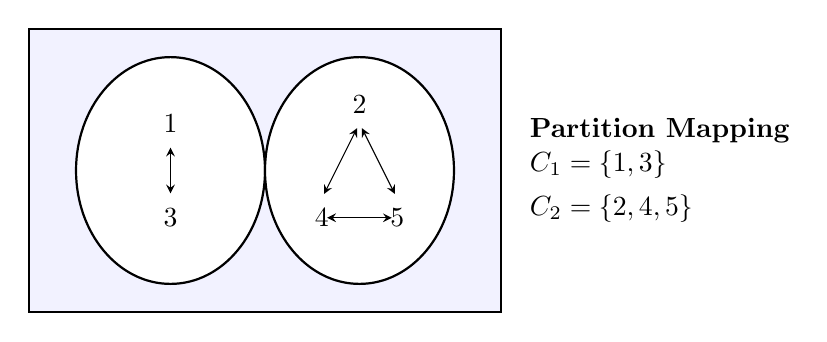
\begin{tikzpicture}[scale=1.2]
        \fill[blue!5] (0,0) rectangle (5,3);
        \draw[thick] (0,0) rectangle (5,3);
        \draw[thick, fill=white] (1.5, 1.5) ellipse (1cm and 1.2cm);
        \draw[thick, fill=white] (3.5, 1.5) ellipse (1cm and 1.2cm);
        
        \node at (1.5, 2) {$1$};
        \node at (1.5, 1) {$3$};
        \draw[<->, >=stealth, shorten >=2pt, shorten <=2pt] (1.5, 1.8) -- (1.5, 1.2);
        
        \node at (3.5, 2.2) {$2$};
        \node at (3.1, 1) {$4$};
        \node at (3.9, 1) {$5$};
        \draw[<->, >=stealth, shorten >=2pt, shorten <=2pt] (3.5, 2.0) -- (3.1, 1.2);
        \draw[<->, >=stealth, shorten >=2pt, shorten <=2pt] (3.5, 2.0) -- (3.9, 1.2);
        \draw[<->, >=stealth, shorten >=2pt, shorten <=2pt] (3.1, 1.0) -- (3.9, 1.0);
        
        \node[align=left, anchor=west] at (5.2, 1.5) {
            \textbf{Partition Mapping}\\
            $C_1 = \{1, 3\}$\\[4pt]
            $C_2 = \{2, 4, 5\}$
        };
    \end{tikzpicture}
\end{proof}

\begin{proof}[Solution to Problem 7]
    \textbf{Technique: Mutual Inclusion via Transitivity.} \\
    Assume $[a] \cap [b] \neq \emptyset$. Then there exists some element $x \in [a] \cap [b]$. By definition of equivalence classes, $x \in [a] \implies xRa$, and $x \in [b] \implies xRb$.
    \begin{itemize}
        \item \textbf{Show $[a] \subseteq [b]$:} Let $y \in [a]$. Then $yRa$. We know $xRa$, which by symmetry implies $aRx$. By transitivity, $yRa$ and $aRx \implies yRx$. We also know $xRb$. By transitivity, $yRx$ and $xRb \implies yRb$. Thus, $y \in [b]$.
        \item \textbf{Show $[b] \subseteq [a]$:} Let $z \in [b]$. Then $zRb$. We know $xRb$, which by symmetry implies $bRx$. By transitivity, $zRb$ and $bRx \implies zRx$. We also know $xRa$. By transitivity, $zRx$ and $xRa \implies zRa$. Thus, $z \in [a]$.
    \end{itemize}
    Since $[a] \subseteq [b]$ and $[b] \subseteq [a]$, we conclude $[a] = [b]$.
\end{proof}

\begin{proof}[Solution to Problem 8]
    \textbf{Technique: Direct Proof on Intersections.} \\
    Let $R = R_1 \cap R_2$.
    \begin{itemize}
        \item \textbf{Reflexivity:} For any $x \in A$, $xR_1x$ and $xR_2x$ because both are reflexive. Thus, $(x,x) \in R_1 \cap R_2 \implies xRx$.
        \item \textbf{Symmetry:} Assume $xRy$. Then $(x,y) \in R_1$ and $(x,y) \in R_2$. Since both are symmetric, $(y,x) \in R_1$ and $(y,x) \in R_2$. Thus, $(y,x) \in R_1 \cap R_2 \implies yRx$.
        \item \textbf{Transitivity:} Assume $xRy$ and $yRz$. Then $(x,y), (y,z) \in R_1$ and $(x,y), (y,z) \in R_2$. Since both are transitive, $(x,z) \in R_1$ and $(x,z) \in R_2$. Thus, $(x,z) \in R_1 \cap R_2 \implies xRz$.
    \end{itemize}
    Therefore, $R_1 \cap R_2$ is an equivalence relation.
\end{proof}

\begin{proof}[Solution to Problem 9]
    \textbf{Technique: Counterexample Construction.} \\
    Let $A = \{1, 2, 3\}$. Define two equivalence relations based on partitions:
    $R_1$ generated by $\{\{1, 2\}, \{3\}\} \implies R_1 = \{(1,1), (2,2), (3,3), (1,2), (2,1)\}$.
    $R_2$ generated by $\{\{1\}, \{2, 3\}\} \implies R_2 = \{(1,1), (2,2), (3,3), (2,3), (3,2)\}$.
    The union is $R_1 \cup R_2 = \{(1,1), (2,2), (3,3), (1,2), (2,1), (2,3), (3,2)\}$.
    Notice that $(1,2) \in R_1 \cup R_2$ and $(2,3) \in R_1 \cup R_2$. If the union were an equivalence relation, it would be transitive, requiring $(1,3) \in R_1 \cup R_2$. However, $(1,3)$ is in neither $R_1$ nor $R_2$. Thus, transitivity fails, and the union is not an equivalence relation.
\end{proof}

\begin{proof}[Solution to Problem 10]
    \textbf{Technique: Combinatorial Partition Counting (Bell Numbers).} \\
    By the Fundamental Theorem, the number of equivalence relations on a set of $n$ elements equals the number of valid partitions of that set (the $n$-th Bell number, $B_n$). For $n=4$, we enumerate the integer partitions of 4 to find the set partitions:
    \begin{itemize}
        \item \textbf{1 block of 4:} $\{\{a,b,c,d\}\}$. There is $\binom{4}{4} = 1$ way.
        \item \textbf{1 block of 3, 1 block of 1:} e.g., $\{\{a,b,c\}, \{d\}\}$. There are $\binom{4}{3} = 4$ ways.
        \item \textbf{2 blocks of 2:} e.g., $\{\{a,b\}, \{c,d\}\}$. There are $\frac{1}{2!} \binom{4}{2}\binom{2}{2} = \frac{6}{2} = 3$ ways.
        \item \textbf{1 block of 2, 2 blocks of 1:} e.g., $\{\{a,b\}, \{c\}, \{d\}\}$. There are $\binom{4}{2} = 6$ ways.
        \item \textbf{4 blocks of 1:} $\{\{a\}, \{b\}, \{c\}, \{d\}\}$. There is $1$ way.
    \end{itemize}
    Total distinct equivalence relations = $1 + 4 + 3 + 6 + 1 = 15$.
\end{proof}

\begin{proof}[Solution to Problem 11]
    \textbf{Technique: Meta-Relational Biconditional Proof.} \\
    \textbf{Forward ($\implies$):} Assume $R$ is an equivalence relation. Then $R$ is reflexive. Let $xRy$ and $xRz$. By symmetry, $yRx$. By transitivity, $yRx \land xRz \implies yRz$. Thus, the property holds. \\
    \textbf{Reverse ($\impliedby$):} Assume $R$ is reflexive and $(xRy \land xRz) \implies yRz$.
    \begin{itemize}
        \item \textbf{Symmetry:} Let $aRb$. Since $R$ is reflexive, $aRa$. Applying the given property with $x=a, y=b, z=a$, we have $(aRb \land aRa) \implies bRa$. Thus, $R$ is symmetric.
        \item \textbf{Transitivity:} Let $aRb$ and $bRc$. Since we just proved $R$ is symmetric, $aRb \implies bRa$. Applying the given property with $x=b, y=a, z=c$, we have $(bRa \land bRc) \implies aRc$. Thus, $R$ is transitive.
    \end{itemize}
    Since $R$ is reflexive, symmetric, and transitive, it is an equivalence relation.
\end{proof}

\begin{proof}[Solution to Problem 12]
    \textbf{Technique: Domain Existence Argument.} \\
    We are given that $R$ is symmetric and transitive. To prove it is an equivalence relation, we only need to prove it is reflexive. Let $x \in A$. By the given domain condition, there exists at least one element $y \in A$ such that $xRy$. Since $R$ is symmetric, $xRy \implies yRx$. We now have the chain $xRy$ and $yRx$. Since $R$ is transitive, $(xRy \land yRx) \implies xRx$. Thus, $R$ is reflexive for all $x \in A$, making it an equivalence relation.
\end{proof}

\begin{proof}[Solution to Problem 13]
    \textbf{Technique: Partition Cardinality.} \\
    By the Partition Theorem, the equivalence classes of $R$ form a partition of $A$. This means the classes $C_1, C_2, \dots, C_m$ are pairwise disjoint and their union is exactly $A$. Therefore, the cardinality of $A$ is the sum of the cardinalities of the distinct equivalence classes:
    \[ |A| = \sum_{i=1}^{m} |C_i| \]
    We are given that $|C_i| = k$ for all $i$. Substituting this into the sum yields:
    \[ |A| = \sum_{i=1}^{m} k = m \cdot k \]
    Since $m$ (the number of distinct classes) is an integer, $k$ divides $|A|$.
\end{proof}

\begin{proof}[Solution to Problem 14]
    \textbf{Technique: Properties of Transitive Closures.} \\
    Let $R^*$ be the transitive closure of $R$. By definition, $R^*$ is transitive, and $x R^* y$ if and only if there exists a finite sequence $a_0, a_1, \dots, a_n$ such that $x = a_0$, $y = a_n$, and $a_{i-1} R a_i$ for all $1 \le i \le n$.
    \begin{itemize}
        \item \textbf{Reflexivity:} Since $R$ is reflexive, $xRx$ for all $x$. Since $R \subseteq R^*$, $x R^* x$.
        \item \textbf{Symmetry:} Assume $x R^* y$. Then there is a path $x R a_1 R a_2 \dots R y$. Since $R$ is symmetric, we can reverse every step: $y R a_{n-1} \dots R a_1 R x$. This forms a valid path from $y$ to $x$ in $R$, meaning $y R^* x$.
    \end{itemize}
    Since $R^*$ is reflexive, symmetric, and transitive, it is an equivalence relation.
\end{proof}

\begin{proof}[Solution to Problem 15]
    \textbf{Technique: Subset Definition of Relations.} \\
    Assume $R \subseteq R^{-1}$. We must show $R$ is symmetric, which means $(x,y) \in R \implies (y,x) \in R$. Let $(x,y) \in R$. Because $R \subseteq R^{-1}$, it follows that $(x,y) \in R^{-1}$. By the definition of the inverse relation, $(x,y) \in R^{-1} \implies (y,x) \in R$. Thus, $R$ is symmetric.
\end{proof}

\begin{proof}[Solution to Problem 16]
    \textbf{Technique: Group Theory Bridge (The Identity Element).} \\
    Let $aRb \iff ab^{-1} \in H$.
    \begin{itemize}
        \item \textbf{Reflexivity:} For any $a \in G$, $aa^{-1} = e$, where $e$ is the identity element. Since $H$ is a subgroup, $e \in H$. Thus, $aRa$.
        \item \textbf{Symmetry:} Assume $aRb$. Then $ab^{-1} \in H$. Since $H$ is a subgroup, it is closed under inverses. Thus, $(ab^{-1})^{-1} \in H$. By group properties, $(ab^{-1})^{-1} = (b^{-1})^{-1}a^{-1} = ba^{-1}$. Since $ba^{-1} \in H$, $bRa$.
        \item \textbf{Transitivity:} Assume $aRb$ and $bRc$. Then $ab^{-1} \in H$ and $bc^{-1} \in H$. Since $H$ is a subgroup, it is closed under the group operation. Thus, $(ab^{-1})(bc^{-1}) \in H$. This simplifies to $a(b^{-1}b)c^{-1} = aec^{-1} = ac^{-1} \in H$. Thus, $aRc$.
    \end{itemize}
    Therefore, $R$ is an equivalence relation (specifically, defining right cosets).
\end{proof}

\begin{proof}[Solution to Problem 17]
    \textbf{Technique: Biconditional Algebraic Proof.} \\
    \textbf{Forward ($\implies$):} Assume $R$ is an equivalence relation. We must show $H$ is a subgroup (closed under addition, contains 0, closed under negation).
    1. Since $R$ is reflexive, $xRx \implies x-x \in H \implies 0 \in H$.
    2. Let $h \in H$. Since $h-0 = h \in H$, $hR0$. By symmetry, $0Rh \implies 0-h \in H \implies -h \in H$.
    3. Let $a, b \in H$. Then $aR0$. Since $b \in H$, by step 2, $-b \in H$, so $0 - (-b) = b \in H \implies 0R(-b)$. By transitivity, $aR0 \land 0R(-b) \implies aR(-b) \implies a - (-b) \in H \implies a+b \in H$. Thus $H$ is a subgroup. \\
    \textbf{Reverse ($\impliedby$):} Assume $H$ is a subgroup.
    1. $0 \in H \implies x-x \in H \implies xRx$.
    2. $xRy \implies x-y \in H$. Since $H$ is closed under negation, $-(x-y) = y-x \in H \implies yRx$.
    3. $xRy \land yRz \implies x-y \in H$ and $y-z \in H$. Since $H$ is closed under addition, $(x-y)+(y-z) = x-z \in H \implies xRz$. Thus $R$ is an equivalence relation.
\end{proof}

\begin{proof}[Solution to Problem 18]
    \textbf{Technique: Well-Definedness via Representative Independence.} \\
    To prove $[a] \cdot [b] = [ab]$ is well-defined, we must show that choosing different representatives for the classes does not change the resulting class. Let $[a] = [a']$ and $[b] = [b']$. This means $a \equiv a' \pmod n$ and $b \equiv b' \pmod n$, so $a - a' = nk$ and $b - b' = nj$ for some $k, j \in \Z$.
    We must show $[ab] = [a'b']$, which requires $ab - a'b'$ to be a multiple of $n$.
    Consider the difference:
    \[ ab - a'b' = ab - a'b + a'b - a'b' = b(a - a') + a'(b - b') \]
    Substitute our initial equations:
    \[ b(nk) + a'(nj) = n(bk + a'j) \]
    Since $(bk + a'j) \in \Z$, $n \mid (ab - a'b')$. Thus, $ab \equiv a'b' \pmod n$, meaning $[ab] = [a'b']$. The operation is well-defined.
\end{proof}

\begin{proof}[Solution to Problem 19]
    \textbf{Technique: Rational Addition Well-Definedness.} \\
    Let $[(a,b)] = [(a',b')]$ and $[(c,d)] = [(c',d')]$. By definition, $ab' = a'b$ and $cd' = c'd$. We must show that $[(ad+bc, bd)] = [(a'd'+b'c', b'd')]$, which requires proving $(ad+bc)b'd' = (a'd'+b'c')bd$.
    Expanding the left-hand side (LHS):
    \[ \text{LHS} = adb'd' + bcb'd' = (ab')dd' + (cd')bb' \]
    Substitute $ab' = a'b$ and $cd' = c'd$:
    \[ \text{LHS} = (a'b)dd' + (c'd)bb' = a'd'bd + b'c'bd = (a'd' + b'c')bd = \text{RHS} \]
    Since the cross-multiplication holds, the resulting equivalence classes are identical. The operation is well-defined.
\end{proof}

\begin{proof}[Solution to Problem 20]
    \textbf{Technique: Function Well-Definedness on Quotients.} \\
    To show $f([x]) = [2x]$ is well-defined, we must prove that if $[x] = [y]$, then $f([x]) = f([y])$.
    Assume $[x] = [y]$. By the definition of the relation, $x - y = 10k$ for some $k \in \Z$.
    We evaluate the outputs: $f([x]) = [2x]$ and $f([y]) = [2y]$. We must show $[2x] = [2y]$, which means $2x - 2y$ must be a multiple of 10.
    \[ 2x - 2y = 2(x - y) = 2(10k) = 20k = 10(2k) \]
    Since $2k \in \Z$, $2x - 2y$ is a multiple of 10. Thus, $[2x] = [2y]$, and the function is well-defined.
\end{proof}

\begin{proof}[Solution to Problem 21]
    \textbf{Technique: Direct Proof (MDP Reward Equivalence).} \\
    Let $s_1 \sim s_2 \iff \forall a \in A, R(s_1, a) = R(s_2, a)$.
    \begin{itemize}
        \item \textbf{Reflexivity:} For any $s \in S$ and $a \in A$, $R(s, a) = R(s, a)$. Thus $s \sim s$.
        \item \textbf{Symmetry:} Assume $s_1 \sim s_2$. Then $\forall a, R(s_1, a) = R(s_2, a) \implies R(s_2, a) = R(s_1, a) \implies s_2 \sim s_1$.
        \item \textbf{Transitivity:} Assume $s_1 \sim s_2$ and $s_2 \sim s_3$. Then $\forall a, R(s_1, a) = R(s_2, a)$ and $R(s_2, a) = R(s_3, a)$. By transitivity of equality, $R(s_1, a) = R(s_3, a) \implies s_1 \sim s_3$.
    \end{itemize}
    Thus, $\sim$ is an equivalence relation.
\end{proof}

\begin{proof}[Solution to Problem 22]
    \textbf{Technique: Affine Transformation Equivalence.} \\
    Let $X \sim Y \iff \exists \alpha > 0, \beta \in \R$ such that $Y = \alpha X + \beta$.
    \begin{itemize}
        \item \textbf{Reflexivity:} $X = 1 \cdot X + 0$. Since $1 > 0$ and $0 \in \R$, $X \sim X$.
        \item \textbf{Symmetry:} Assume $X \sim Y$. Then $Y = \alpha X + \beta$ for $\alpha > 0$. Solving for $X$ yields $X = \frac{1}{\alpha}Y - \frac{\beta}{\alpha}$. Since $\alpha > 0$, $\frac{1}{\alpha} > 0$. Let $\alpha' = \frac{1}{\alpha}$ and $\beta' = -\frac{\beta}{\alpha}$. Then $X = \alpha' Y + \beta'$, so $Y \sim X$.
        \item \textbf{Transitivity:} Assume $X \sim Y$ and $Y \sim Z$. Then $Y = \alpha_1 X + \beta_1$ and $Z = \alpha_2 Y + \beta_2$ ($\alpha_1, \alpha_2 > 0$). Substituting $Y$ into $Z$ gives $Z = \alpha_2(\alpha_1 X + \beta_1) + \beta_2 = (\alpha_2 \alpha_1)X + (\alpha_2 \beta_1 + \beta_2)$. Since $\alpha_1 > 0$ and $\alpha_2 > 0$, their product $\alpha_2 \alpha_1 > 0$. Thus, $X \sim Z$.
    \end{itemize}
    Thus, $\sim$ is an equivalence relation.
\end{proof}

\begin{proof}[Solution to Problem 23]
    \textbf{Technique: Measure Theory and Symmetric Differences.} \\
    Let $A \sim B \iff \Prob(A \triangle B) = 0$.
    \begin{itemize}
        \item \textbf{Reflexivity:} $A \triangle A = (A \setminus A) \cup (A \setminus A) = \emptyset$. Since $\Prob(\emptyset) = 0$, $A \sim A$.
        \item \textbf{Symmetry:} $A \triangle B = (A \setminus B) \cup (B \setminus A) = (B \setminus A) \cup (A \setminus B) = B \triangle A$. Thus $\Prob(A \triangle B) = \Prob(B \triangle A) = 0 \implies B \sim A$.
        \item \textbf{Transitivity:} Assume $A \sim B$ and $B \sim C$. We use the set-theoretic property $A \triangle C \subseteq (A \triangle B) \cup (B \triangle C)$. By the monotonicity and subadditivity of probability measures:
        \[ \Prob(A \triangle C) \le \Prob((A \triangle B) \cup (B \triangle C)) \le \Prob(A \triangle B) + \Prob(B \triangle C) \]
        Substituting our assumptions: $\Prob(A \triangle C) \le 0 + 0 = 0$. Since probability cannot be negative, $\Prob(A \triangle C) = 0 \implies A \sim C$.
    \end{itemize}
    Thus, $\sim$ is an equivalence relation.
\end{proof}

\begin{proof}[Solution to Problem 24]
    \textbf{Technique: Set-Theoretic Bounds on Probability.} \\
    Assume $A_1 \sim B_1$ and $A_2 \sim B_2$. This means $\Prob(A_1 \triangle B_1) = 0$ and $\Prob(A_2 \triangle B_2) = 0$. We must show $(A_1 \cup A_2) \sim (B_1 \cup B_2)$, which requires $\Prob((A_1 \cup A_2) \triangle (B_1 \cup B_2)) = 0$.
    By standard set theory, the symmetric difference of unions is bounded by the union of symmetric differences:
    \[ (A_1 \cup A_2) \triangle (B_1 \cup B_2) \subseteq (A_1 \triangle B_1) \cup (A_2 \triangle B_2) \]
    Applying the probability measure and subadditivity:
    \[ \Prob((A_1 \cup A_2) \triangle (B_1 \cup B_2)) \le \Prob(A_1 \triangle B_1) + \Prob(A_2 \triangle B_2) = 0 + 0 = 0 \]
    Thus, the union operation is well-defined on these equivalence classes.
\end{proof}

\begin{proof}[Solution to Problem 25]
    \textbf{Technique: Counterexample to Transitivity (Tolerance Relations).} \\
    Let $x \sim y \iff \|f(x) - f(y)\| \le \epsilon$. While this relation is reflexive (distance is 0) and symmetric (norm is absolute), it fails transitivity.
    \textbf{Counterexample:} Choose points $x, y, z$ such that $f(x) = 0$, $f(y) = \epsilon$, and $f(z) = 2\epsilon$.
    Then $\|f(x) - f(y)\| = \epsilon \le \epsilon \implies x \sim y$.
    And $\|f(y) - f(z)\| = \epsilon \le \epsilon \implies y \sim z$.
    However, $\|f(x) - f(z)\| = 2\epsilon \not\le \epsilon$. Thus $x \not\sim z$.
    Because transitivity fails, $\sim$ is a tolerance relation, not an equivalence relation.
\end{proof}

\begin{proof}[Solution to Problem 26]
    \textbf{Technique: Identifying Division by Zero.} \\
    \textbf{The Flaw:} The proof divides the inequality $xy^2z \ge 0$ by $y^2$. If $y = 0$, this division is undefined, and the deduction $xz \ge 0$ is invalid.
    \textbf{Counterexample:} Let $x = -1, y = 0, z = 1$.
    $xRy$ holds because $-1 \cdot 0 = 0 \ge 0$.
    $yRz$ holds because $0 \cdot 1 = 0 \ge 0$.
    However, $xRz$ fails because $-1 \cdot 1 = -1 < 0$. Thus, the relation is not transitive.
\end{proof}

\begin{proof}[Solution to Problem 27]
    \textbf{Technique: Identifying the Empty Domain / Reflexivity Failure.} \\
    \textbf{The Flaw:} The student correctly identifies that transitivity fails, but incorrectly concludes it is "an equivalence relation that just lacks transitivity." An equivalence relation MUST possess all three properties. Furthermore, the student completely skipped checking reflexivity.
    \textbf{Counterexample to Reflexivity:} Let $x = 1$. $x+x = 1+1 = 2$, which is even. Thus $1 \not R 1$. The relation is not reflexive.
\end{proof}

\begin{proof}[Solution to Problem 28]
    \textbf{Technique: Edge Case Analysis (The Empty Set).} \\
    \textbf{The Flaw:} The proof claims $A \cap A = A \neq \emptyset$ for "any set $A$". This is false for the empty set.
    \textbf{Counterexample:} Let $A = \emptyset$. Then $\emptyset \cap \emptyset = \emptyset$. Thus, $\emptyset \not R \emptyset$. The relation is not reflexive on the power set.
\end{proof}

\begin{proof}[Solution to Problem 29]
    \textbf{Technique: Definition of a Partition.} \\
    \textbf{The Flaw:} The collection $P = \{\{1, 2\}, \{2, 3\}\}$ is NOT a valid partition. By definition, the subsets in a partition must be pairwise disjoint.
    \textbf{Counterexample:} $\{1, 2\} \cap \{2, 3\} = \{2\} \neq \emptyset$. Because the sets overlap, they do not form a partition, and the Fundamental Theorem cannot be applied.
\end{proof}

\begin{proof}[Solution to Problem 30]
    \textbf{Technique: Logical Fallacy in Reciprocals.} \\
    \textbf{The Flaw:} The proof states "if $y/x$ is an integer... this implies $x/y$ is an integer." This is mathematically false for almost all integers.
    \textbf{Counterexample:} Let $x = 2$ and $y = 4$. $2 \mid 4$ because $4/2 = 2 \in \Z$. Thus $2R4$. However, $4 \nmid 2$ because $2/4 = 0.5 \notin \Z$. Thus $4 \not R 2$. The relation is not symmetric (it is actually a partial order).
\end{proof}

\newpage

\section{Concept Checklist \& Question Mapping (Reference)}

\vspace{1em}
\renewcommand{\arraystretch}{1.5}
\noindent
\begin{tabularx}{\textwidth}{l X l}
\toprule
\textbf{ID} & \textbf{Concept / Proof Technique} & \textbf{Associated Problems} \\
\midrule
C1 & Abstract Property Verification (Reflexivity, Symmetry, Transitivity) & 1, 2, 3, 4, 5 \\
C2 & Partition Mapping \& Equivalence Classes & 6, 7, 8, 9, 10 \\
C3 & Combinatorial \& Meta-Relational Arguments & 11, 12, 13, 14, 15 \\
C4 & The ``Zero-Addition'' Trick \& Algebraic Bridges & 16, 17 \\
C5 & Parity and Divisibility Translation & 1, 4, 20 \\
C6 & Symmetry as a Path-Reverser & 11, 12, 14 \\
C7 & Well-Defined Operations on Quotient Sets & 18, 19, 20 \\
C8 & Real-World Modeling (MDP Bisimulation, Asset Clustering, ML) & 21, 22, 23, 24, 25 \\
C9 & Diagnostic Testing / Finding Flaws (Empty Domain, Div by Zero) & 26, 27, 28, 29, 30 \\
\bottomrule
\end{tabularx}
\vspace{1em}

\end{document}